% safe参数解决与\!在内的多个冲突
% \sups命令可能被重定义,xeCJK放在tipa后
\RequirePackage[safe]{tipa}

\documentclass[a4paper, zihao=-4, linespread=1]{ctexrep}
\renewcommand{\CTEXthechapter}{\thechapter}
% 最小行间间距设定
\setlength{\lineskiplimit}{3pt}
\setlength{\lineskip}{3pt}

% 中文支持
\setCJKmainfont[BoldFont=SourceHanSerifCN-Bold.otf]{SourceHanSerifCN-Regular.otf} 
  \xeCJKsetup{CJKmath=true}
  \setCJKmathfont{KaiTi}  % 数学环境中使用楷体
\newCJKfontfamily[zhxinwei]\xinwei{STXinwei} % 定义新字体

% 颜色
\usepackage[table]{xcolor}
  \newcommand{\scol}[1]{\colorbox{#1}{\rule{0em}{1ex}}\,#1}
  
% 首字下沉
\usepackage{lettrine}

% 分栏
\usepackage{multicol}
  \setlength{\columnsep}{20pt}
  \setlength{\columnseprule}{0.4pt}

% 数学环境
\usepackage{mathdots} % 数学省略号,会重定义 dddot 和 ddddot
\usepackage{amsmath}  
  \newcommand{\ue}{\mathrm{e}}
  \newcommand{\ud}{\mathop{}\negthinspace\mathrm{d}} % 微分号
\usepackage{amssymb}
\usepackage{mathrsfs} % 线性代数字体
% overline的替代命令
\newcommand{\closure}[2][3]{{}\mkern#1mu\overline{\mkern-#1mu#2}}
\usepackage{yhmath} % \wideparen命令:弧AB
\usepackage{mathtools} % dcases环境,prescript命令
\usepackage{amsthm} % 定理环境
  \theoremstyle{definition}\newtheorem{laws}{Law}[section]
  \theoremstyle{plain}\newtheorem{ju}[laws]{Jury}
  \theoremstyle{remark}\newtheorem*{marg}{Margaret}
\usepackage{esint} % 多重积分,需放在amsmath后
% 箭头与长等号
\usepackage{extarrows}
% 中括号的类二项式命令
\newcommand{\Bfrac}[2]{\genfrac{[}{]}{0pt}{}{#1}{#2}}

% 下划线宏包
\usepackage[normalem]{ulem}
% LaTeX符号宏包
\usepackage{hologo}
	\newcommand{\xelatex}{\Hologo{XeLaTeX}}
	\newcommand{\bibtex}{\Hologo{BibTeX}}
	\newcommand{\tikzz}{Ti\textit{k}Z}
	\newcommand{\bz}{B\'ezier}
% 其他符号
\usepackage{wasysym}
% 带箱小页
\usepackage{boxedminipage}
% 绘图
\usepackage{tikz}
  \usetikzlibrary{calc,intersections,positioning,angles,quotes,decorations.pathmorphing,fit,backgrounds,through}
  \newcommand{\tikzline}[1]{{#1\tikz{\draw[#1,line width=9](0,0)--(0.5,0);}}, }
% 最后一页
\usepackage{lastpage}

% 奇怪的小定义
\newcommand{\dpar}{\\ \mbox{}}  % 空两行
\newcommand{\qd}[1]{{\bfseries{#1}}}  % 强调
\newcommand{\co}[1]{{\bfseries{#1}}}  % Style of concept
\newcommand{\RED}[1]{{\color{cyan}{#1}}}
\newcommand{\cmmd}[1]{\fbox{\texttt{\char92{}#1}}}
\newcommand{\charef}[1]{第\ref{#1}章}
\newcommand{\secref}[1]{第\ref{#1}节}
\newcommand{\pref}[1]{第\pageref{#1}页}
\newcommand{\fref}[1]{图\ref{#1}}
\newcommand{\tref}[1]{表\ref{#1}}

% Quote 环境
\newenvironment{QuoteEnv}[2][]
    {\newcommand\Qauthor{#1}\newcommand\Qref{#2}}
    {\medskip\begin{flushright}\small ——~\Qauthor\\
    \emph{\Qref}\end{flushright}}
% 字体调用
\newcommand{\myfont}[2]{{\fontfamily{#1}\selectfont #2}}

% 编号列表宏包,并自定义了三个列表
\usepackage[inline]{enumitem}
	\setlist[enumerate]{font=\bfseries,itemsep=0pt}
	\setlist[itemize]{font=\bfseries,leftmargin=\parindent}
	\setlist[description]{font=\bfseries\uline}

\newenvironment{fead}{	
    \begin{description}[font=\bfseries\uline,labelindent=\parindent,itemsep=0pt,parsep=0pt,topsep=0pt,partopsep=0pt]}
	{\end{description}}
% 带宽度的
\newenvironment{para}{
	\begin{description}[font=\bfseries\ttfamily,itemsep=0pt,parsep=0pt,topsep=0pt,partopsep=0pt]}
	{\end{description}}
\newenvironment{feae}{
	\begin{enumerate}[font=\bfseries,labelindent=0pt,itemsep=0pt,parsep=0pt,topsep=0pt,partopsep=0pt]}
	{\end{enumerate}}
\newenvironment{feai}{
	\begin{itemize}[font=\bfseries,itemsep=0pt,parsep=0pt,topsep=0pt,partopsep=0pt]}
	{\end{itemize}}
\newenvironment{inlinee}
{\begin{enumerate*}[label=(\arabic*), font=\rmfamily, before=\unskip{:},itemjoin={{;}},itemjoin*={{,以及:}}]}
	{\end{enumerate*}。}

% 目录和章节样式
\usepackage{titlesec}
\usepackage{titletoc}   % 用于目录

\titlecontents{chapter}[1.5em]{}{\contentslabel{1.5em}}{\hspace*{-2em}}{\hfill\contentspage}
\titlecontents{section}[3.3em]{}{\contentslabel{1.8em}}
	{\hspace*{-2.3em}}{\titlerule*[8pt]{$\cdot$}\contentspage}
\titlecontents*{subsection}[2.5em]{\small}{\thecontentslabel{} }{}{, \thecontentspage}[;\qquad][.]
% 章节样式
\setcounter{secnumdepth}{3} % 一直到subsubsection
\newcommand{\chaformat}[1]{%
	\parbox[b]{.5\textwidth}{\hfill\bfseries #1}%
	\quad\rule[-12pt]{2pt}{70pt}\quad
	{\fontsize{60}{60}\selectfont\thechapter}}
\titleformat{\chapter}[block]{\hfill\LARGE\sffamily}{}{0pt}{\chaformat}[\vspace{2.5pc}\normalsize
	\startcontents\setlength{\lineskiplimit}{0pt}\printcontents{}{1}{\setcounter{tocdepth}{2}\songti}]
\titleformat*{\section}{\centering\Large\bfseries}
\titleformat{\subsubsection}[hang]{\bfseries\large}{\rule{1.5ex}{1.5ex}}{0.5em}{}
% 扩展章节
\newcommand{\starsec}{\noindent\fbox{\S\textit{注意:本章节是一个扩展阅读章节。}}
	\\ \mbox{}}

\renewcommand{\contentsname}{目录}
	\renewcommand{\tablename}{表}
	\renewcommand\arraystretch{1.2}	% 表格行距
	\renewcommand{\figurename}{图}
% 设置不需要浮动体的表格和图像标题
\setlength{\abovecaptionskip}{5pt}
\setlength{\belowcaptionskip}{3pt}
\makeatletter
\newcommand\figcaption{\def\@captype{figure}\caption}
\newcommand\tabcaption{\def\@captype{table}\caption}
\makeatother
% 图表
\usepackage{array,multirow,makecell}
  \setlength\extrarowheight{2pt} % 行高增加
\usepackage{diagbox}
\usepackage{longtable}
\usepackage{graphicx,wrapfig}
  \graphicspath{{./tikz/}}
\usepackage{animate}
\usepackage{caption,subcaption}
  \captionsetup[sub]{labelformat=simple}
  \renewcommand{\thesubtable}{(\alph{subtable})}
% 三线表
\usepackage{booktabs}  

% 页面修正宏包
\usepackage{geometry}
  \geometry{vmargin = 1in}

% 代码环境
\usepackage{listings}
% 复制代码时不复制行号
\usepackage{accsupp}
	\newcommand{\emptyaccsupp}[1]{\BeginAccSupp{ActualText={}}#1\EndAccSupp{}}
\usepackage{tcolorbox}
  \tcbuselibrary{listings,skins,breakable,xparse}

% global style
\lstset{
  basicstyle=\small\ttfamily,
  % Word styles
  keywordstyle=\color{blue},
  commentstyle=\color{green!50!black},
  columns=fullflexible,  % Avoid too sparse word spaces
  keepspaces=true,
  % Numbering
  numbers=left,
  numberstyle=\tiny\color{red!75!black}\emptyaccsupp,
  % Lines and Skips
  aboveskip=0pt plus 6pt,
  belowskip=0pt plus 6pt,
  breaklines=true,
  breakatwhitespace=true,
  emptylines=1,  % Avoid >1 consecutive empty lines
  escapeinside=``
}

% TikZ Language Hint
\lstdefinelanguage{tikzlang}{
  sensitive=true,
  morecomment=[n]{[}{]}, % nested comment
  morekeywords={
    draw,clip,filldraw,path,node,coordinate,foreach,pic,
    tikzset
  }
}

% 对于 tcolorbox 中 listings 库的 ''tcblatex'' style 的重现,
% 添加了新的关键词
\lstdefinestyle{latexcn}{
  language=[LaTeX]TeX,
  % More Keywords
  classoffset=0,
  texcsstyle=*\color{blue},
  moretexcs={
    % LaTeX extension
    chapter,section,subsection,setlength,
    thechapter,thesection,thesubsection,theequation,
    chaptermark,chaptername,appendix,
    bibname,refname,bibpreamble,bibfont,citenumfont,bibnumfmt,bibsep,
  },
  classoffset=1,
  texcsstyle=*\color{orange!75!black},
  moretexcs={
    % XeCJK & CTeX
    xeCJKsetup,setCJKmainfont,newCJKfontfamily,CJKfontspec,
    CTEXthechapter,songti,heiti,fangsong,kaishu,yahei,lishu,youyuan,
    % AMSmath / AMSsymb / AMSthm
    middle,text,tag,boldsymbol,mathbb,dddot,ddddot,iint,varoiint,
    dfrac,tfrac,cfrac,leftroot,uproot,underbracket,xleftarrow,xrightarrow,
    overset,underset,sideset,mathring,leqslant,geqslant,because,therefore,
    shortintertext,binom,dbinom,implies,thesubequation,
    impliedby,genfrac,theoremstyle,qedhere,
    % Other math packages
    wideparen,intertext,
    xlongequal,xLeftrightarrow,xleftrightarrow,xLongleftarrow,xLongrightarrow,
    % xcolor
    definecolor,color,textcolor,colorbox,fcolorbox,
    % hyperref
    hyperref,autoref,href,url,nolinkurl,
    % Graph & Table
    includegraphics,graphicspath,scalebox,rotatebox,animategraphics,
    newcolumntype,arraybackslash,multirow,captionsetup,
    thead,multirowcell,makecell,Xhline,Xcline,diagbox,
    toprule,midrule,bottomrule,DeclareFloatingEnvironment,
    % ulem
    uline,uuline,dashuline,dotuline,uwave,sout,xout,
    % fancyhdr
    lhead,chead,rhead,lfoot,cfoot,rfoot,
    fancyhf,fancyhead,fancyfoot,fancypagestyle,
    % fontspec
    newfontfamily,
    % titlesec & titletoc
    titlelabel,titleformat,titlespacing,titleline,titlerule,dottecontents,titlecontents,
    % enumitem
    setlist,
    % Listings & tcolorbox
    lstdefinelanguage,lstdefinestyle,lstset,lstnewenvironment,
    tcbuselibrary,newtcblisting,newtcbox,DeclareTCBListing
    % citation & index: natbib, imakeidx
    setcitestyle,printindex,
    % Other packages
    hologo,lettrine,endfirsthead,endhead,endlastfoot,columncolor,rowcolors,modulolinenumbers,MakeShortVerb,tikz
  }
}

% cmd & envi
\newtcbox{\latexline}[1][green]{on line,before upper=\ttfamily\char`\\,
  arc=0pt,outer arc=0pt,colback=#1!10!white,colframe=#1!50!black,
  boxsep=0pt,left=1pt,right=1pt,top=1pt,bottom=1pt,
  boxrule=0pt,bottomrule=1pt,toprule=1pt}
\newtcbox{\envi}[1][violet!70!cyan]{on line,before upper=\ttfamily,
  arc=0pt,outer arc=0pt,colback=#1!10!white,colframe=#1!50!black,
  boxsep=0pt,left=1pt,right=1pt,top=1pt,bottom=1pt,
  boxrule=0pt,bottomrule=1pt,toprule=1pt}
% pkg
\newtcbox{\pkg}[1][orange!70!red]{on line,before upper={\rule[-0.2ex]{0pt}{1ex}\ttfamily},
  arc=0.8ex,colback=#1!30!white,colframe=#1!50!black,
  boxsep=0pt,left=1.5pt,right=1.5pt,top=1pt,bottom=1pt,
  boxrule=1pt}
\newcommand{\tikzkw}[1]{\texttt{#1}}

% tcblisting definitions
\newtcblisting{latex}{breakable,skin=bicolor,colback=gray!30!white,
  colbacklower=white,colframe=cyan!75!black,listing only, 
  left=6mm,top=2pt,bottom=2pt,fontupper=\small,
  listing options={style=latexcn}
}

\NewTCBListing{codeshow}{ O{listing side text} }{
  skin=bicolor,colback=gray!30!white,
  colbacklower=pink!50!yellow,colframe=cyan!75!black,
  halign lower=center,valign lower=center,
  left=6mm,righthand width=0.4\linewidth,fontupper=\small,
  % listing style
  listing options={style=latexcn},#1,
}

% Fix solution from the tcolorbox package author
\makeatletter
\tcbset{
  tikz upper/.style={before upper=\centering\tcb@shield@externalize\begin{tikzpicture}[{#1}],after upper=\end{tikzpicture}},%
  tikz lower/.style={before lower=\centering\tcb@shield@externalize\begin{tikzpicture}[{#1}],after lower=\end{tikzpicture}},%
}
\makeatother

% xparse library required
\NewTCBListing{tikzshow}{ O{} }{
  tikz lower={#1},
  halign lower=center,valign lower=center,
  skin=bicolor,colback=gray!30!white,
  colbacklower=white,colframe=cyan!75!black, 
  left=6mm,righthand width=3.5cm,listing outside text,
  listing options={language=tikzlang}
}

\NewTCBListing{tikzshowenvi}{ O{} }{
  halign lower=center,valign lower=center,
  skin=bicolor,colback=gray!30!white,
  colbacklower=white,colframe=cyan!75!black, 
  left=6mm,righthand width=3.5cm,listing outside text,
  listing options={language=tikzlang},#1
}
% inline tikz draw
%\newcommand{\tikzline}{def}

% 附录
% \usepackage{appendix}
\renewcommand{\appendixname}{App.}

% 行号
\usepackage{lineno}

% 索引与参考文献
\usepackage{imakeidx}
  \newcommand{\tikzidx}[1]{\index{\char`\\ #1}}
  \newcommand{\tikzoptstyle}[1]{\texttt{#1}}
  \newcommand{\tikzopt}[2][draw]{\tikzoptstyle{#2}\index{\char`\\ #1!#2}\ }
  \renewcommand{\indexname}{\tikzz 命令索引}
\makeindex[intoc]

\bibliographystyle{plain}
\renewcommand{\bibname}{参考文献}
\usepackage[numindex,numbib]{tocbibind}
\usepackage[square,super,sort&compress]{natbib}

% 引用
\usepackage{hyperref}
\hypersetup{colorlinks, bookmarksopen = true, bookmarksnumbered = true, pdftitle=LaTeX-cn, pdfauthor=K.L Wu, pdfstartview=FitH}


\title{Learn \LaTeX{} by Examples}
\author{Kanglong Wu}

\begin{document}
	
\maketitle

\tableofcontents

\chapter{序}

\noindent{\Huge\CJKfontspec{STXinwei} 第一稿序}\dpar\dpar

其实在之前我是有一稿手册的,开始撰写的日期大概在2015年4月。但是自己觉得写得太烂,因此索性推倒重写了这一版。这一版的主要特征是:
\begin{feae}
	\item 我希望能够吸引初学者快速上手,解决手头的问题。因此去掉了枯燥的讲解和无穷无尽的宏包用法介绍,直接使用实例;
	\item 力求突出实用性。当然,也会提点一些可以深入学习的内容,读者可以自行查阅,或者阅读本手册中的扩展阅读章节(即带星号*的章节)。
	\item 本手册使用的编辑器为\TeX Studio,而非之前的商业软件WinEdt. 这使得学习\LaTeX 的门槛更低。当然了,你有权使用任何编辑器,我并不是说\TeX Studio就是最好的。事实上在你熟练以后,使用记事本+命令行的方式生成文档都是没有问题的。
\end{feae}

由于工作全部由我一人完成,限于视野,难免存在错漏之处。恳请读者指正。有任何使用中遇到的手册中无法解决的问题,欢迎向我提出。

\vfill

\begin{flushright}
Mail: wklchris@hotmail.com\dpar

Chris Wu

\today 于湖北
\end{flushright}



\chapter{\LaTeX{}基础}
\section{第一份文稿}

编辑器的配置大概是需要讲解一下的,毕竟对于初学者来说是很头疼的事情。本手册就以\TeX Studio为例进行配置。首先你应该安装一个\TeX{} Live,它是完全免费的,网址:\url{http://tug.org/texlive/}. 

虽然它体积较大,但是却是最一劳永逸、最不需要花时间取配置的方法,同时它大概也是功能支持最强的\LaTeX 发行版。

打开\TeX Studio后,选择选项$\rightarrow$ 设置\TeX Studio $\rightarrow$ 构建$\rightarrow$ 默认编译器,选择\xelatex{}. 这主要是基于中文文档编译的考虑,同时\xelatex 也能很好地编译英文文档。我建议始终使用它作为默认编译器。\dpar

之后你可以在编译窗口输入一篇小文档,并保存为tex文件进行测试:
\begin{latex}{}
\documentclass{article}
\usepackage[slantfont,boldfont]{xeCJK}
\setCJKmainfont[BoldFont=SimHei,ItalicFont=KaiTi]{SimSun}
\begin{document}
	Hello, world!
	你好,世界!
\end{document}
\end{latex}

点击编译按钮生成,F7查看。生成的pdf在你的tex文件保存目录中。具体各行的含义我们会在后文介绍。

\section{认识\LaTeX}
\subsection{命令与环境}
\LaTeX 中的\co{命令}通常是由一个反斜杠加上命令名称,再加上花括号内的参数构成的。比如:

\begin{latex}{}
\documentclass{article}
\end{latex}

如果有一些选项是备选的,那么通常会在花括号前用方括号标出。比如:

\begin{latex}{}
\documentclass[a4paper]{article}
\end{latex}

在\LaTeX 中,还有一种重要的指令叫做\co{环境}。它定义了一整个区段的内容都受到环境(即其本身)的控制。这个区段是从\cmmd{begin\{{\itshape environment}\}}开始,到\cmmd{end\{{\itshape environment\}}}结束的。。比如:

\begin{latex}{}
\begin{document}
	...内容...
\end{document}
\end{latex}

同样的,环境也可以使用备选选项,只需要写在begin的后面就行了。

注意:不带花括号的命令后面如果想打印空格,请加上\RED{一对内部为空的花括号}再键入空格。否则空格会被忽略。例如:\verb+\LaTeX{} Studio+. 

\subsection{保留字符}

\LaTeX 中有许多字符有着特殊的含义,在你生成文档时不会直接打印。例如每个命令的第一个字符:反斜杠。单独输入一个反斜杠在你的行文中不会有任何帮助,甚至可能产生错误。\LaTeX 中的保留字符有:
\begin{center}
\texttt{\# \$ \% \^ \& \_ \{ \} \char92}
\end{center}

以上除了反斜杠外,均能用前加反斜杠的行驶输出。即你只需要键入:
\begin{center}
\texttt{\char92{}\# \char92{}\$ \char92{}\% \char92{}\^{} \char92{}\& \char92{}\_
	\char92{}\{ \char92{}\} }
\end{center}

唯独反斜杠的输出比较头痛,你可以尝试:
\begin{verbatim}
$\backslash$
\texttt{\char92}
\end{verbatim}

另外需要说明的是,在中文格式下,波浪线{\texttt{\~}}用来输出一个小空格,不能够直接输出。你可以通过命令\verb+$\sim$+来产生一个。

\subsection{导言区}
任何一份\LaTeX{}文档都应当包含以下结构:

\begin{latex}{}
\documentclass[`\itshape options`]{doc-class}
\begin{document}
	...
\end{document}
\end{latex}

其中,在语句\latexline{\\begin{document}}之前的内容称为\co{导言区}。导言区可以留空,以可以进行一些文档的准备操作。你可以粗浅地理解为:\RED{导言区即模板定义}。\dpar

文档类的参数doc-class和可选选项{\textit{options}}有以下取值:
\begin{center}
	\tabcaption{文档类和选项}
	\label{tb:documentclass}
	\begin{tabular}{p{5em} @{\ -\ } p{24em}}
		\hline
		\multicolumn{2}{l}{\bfseries doc-class文档类} \\
		\hline
		article   & 科学期刊,演示文稿,短报告,邀请函。\\
		proc      & 基于article的会议论文集。\\
		report    & 多章节的长报告、博士论文、短篇书。\\
		book      & 书籍。\\
		slides    & 幻灯片,使用了大号Scans Serif字体。\\
		\hline
		\multicolumn{2}{l}{\bfseries\itshape options} \\
		\hline
		字体     & 默认10pt\\
		页面方向 & 默认竖向portrait,可选横向landscape。\\
		纸张尺寸 & 默认letterpaper,可选用a4paper, b5paper等。\\
		分栏     & 默认onecolumn,还有twocolumn。\\
		双面打印 & 有oneside/twoside两个选项,用于排版奇偶页。article/report默认单面。\\
		章节分页 & 有openright/openany两个选项,决定是在奇数页开启新页或是任意页开启新页。注意article是没有chapter(``章'')命令的,默认任意页。\\
		公式对齐 & 默认居中,可改为左对齐fleqn;默认编号居右,可改为左对齐leqno。\\
		\hline
	\end{tabular}
\end{center}

在本文中,多数的文档类提及的均为report/book类。如果有article类将会特别指明。其余的文档类不予说明。本手册排版即使用了book类。\dpar

在导言区最常见的是\co{宏包}的加载工作,命令形如:\latexline{\\usepackage{package}}。通俗地讲,宏包是指一系列已经制作好的功能``模块'',在你需要使用一些原生\LaTeX 不带有的功能时,只需要调用这些宏包就可以了。比如本文的代码就是利用{\texttt{listings}}宏包实现的。

宏包的具体使用将参在各部分内容说明中进行讲解。

\subsection{错误的查找}
\label{subsec:debug}
在编辑器界面上,下方的日志是显示编译过程的地方。在你编译通过后,会出现这样的字样:
\begin{feai}
	\item {\qd{Errors错误}}:严重的错误。一般地,编译若通过了,该项是零。
	\item {\qd{Warnings警告}}:一些不影响生成文档的瑕疵。
	\item {\qd{Bad Boxes坏箱}\footnote{Box是\LaTeX{}中的一个特殊概念,具体将在\protect\secref{sec:box}部分进行讲解。}}:指排版中出现的长度问题,比如长度超出(Overfull)等。后面的Badness表示错误的严重程度,程度越高数值越大。这类问题需要检查,排除Badness高的选项。
\end{feai}

你可以向上翻阅控制台记录,来找到Warning开头的记录,或者Overfull/ Underfull开头的记录。这些记录会指出你的问题出在哪一行(比如line 1-2) 或者在输出pdf的哪一页(比如active [12]。注意,这个12表示页面显示页码或者计数器计数页码,而不是文件打印出来的真实页码)。此外你可以还需要了解:
\begin{feai}
	\item 值得指出的是,由于\LaTeX{}的编译原理(第一次生成aux文件,第二次再引用它),目录想要合理显示\qd{需要连续编译两次}。在连续编译两次后,你会发现一些Warnings会在第二次编译后消失。在\TeX Studio中,你可以只单击一次“构建并查看”,它会检测到文章的变化并自动决定是否需要编译两次。
	\item 对于大型文档,寻找行号十分痛苦。你需要学会合理地拆分tex文件,参阅\secref{sec:include}的内容。
\end{feai}
\subsection{文件输出}
\LaTeX{}的输出一般推荐pdf格式,由\LaTeX 直接生成dvi的方法并不推荐。

你在tex文档的文件夹下可能看到的其他文件类型:
\begin{tabbing}
	.sty{\hspace{2em}}\=宏包文件\\
	.aux    \> 用于储存交叉引用信息的文件。因此,在更新交叉引用(公式编号、\\
	\> 大纲级别)后,需要编译两次才能正常显示。\\
	.log    \> 记录上次编译的信息。\\
	.toc    \> 目录文件。\\
	.idx    \> 如果文档中包含索引,该文件用于储存索引信息。\\
	.lof    \> 图形目录。\\
	.lot    \> 表格目录。
\end{tabbing}

有时\LaTeX 的编译出现异常,你需要删除文件夹下除了tex以外的文件再编译。此外,在某些独占程序打开了以上的文件时(比如用Acrobat打开了pdf),编译可能出现错误。请在编译时确保关闭这些独占程序。

\section{标点符号}
\subsection{引号}
单引号并不使用两个\verb|'|符号组合。左单引号是重音符\verb|`|(键盘上数字1左侧),而右单引号是常用的引号符。英文中,\RED{左双引号就是连续两个重音符}。

英文下的引号嵌套需要借助\verb|\thinspace|命令分隔,比如:

\begin{codeshow}
``\thinspace`Max' is here.''
\end{codeshow}

中文下的单引号和双引号你可以用中文输入法直接输入。

\subsection{破折与短横}
英文的短横分为三种:
\begin{feai}
\item 连字符:输入一个短横:\verb|-|,效果如daughter-in-law
\item 数字起止符:输入两个短横:\verb|--|,效果如:page 1--2
\item 破折号:输入三个短横:\verb|---|,效果如:Listen---I'm serious.
\end{feai}

中文的破折号你也许可以直接使用日常的输入方式。

至于减号,也许你应该借助于数学环境来输入:\verb|$-$|. 

\subsection{强调:粗与斜}
\LaTeX 中专门有个叫做\latexline{\em{text}}的命令,可以强调文本。对于通常的西文文本,上述命令的作用就是斜体。如果你对一段已经这样转换为斜体的文本再使用这个命令,它就会取消斜体,而成为正体。

西文中一般采用上述的斜体强调方式而不是粗体,例如在说明书名的时候就会使用以上命令。关于字体的更多内容参考\hyperref[sec:font]{字体}这一节。

\subsection{下划线与删除线}
\LaTeX 原生提供了\latexline{\underline}命令简直烂的可以,建议你使用ulem宏包下的\texttt{uline}命令代替。ulem宏包还提供了一系列有用的命令:

\begin{codeshow}
\uline{下划线} \\
\uuline{双下划线} \\
\dashuline{虚下划线} \\
\dotuline{点下划线} \\
\uwave{波浪线} \\
\sout{删除线} \\
\xout{斜删除线}
\end{codeshow}

需要注意的是,ulem宏包重定义了\verb|\emph|命令,\RED{使得原来的加斜强调变成了下划线、原来的两次强调就取消强调变成了两次强调就双下划线},同时也支持换行文本。

\subsection{其他}
角度符号或者温度符号需要借助数学模式\verb|$...$|输入:

\begin{codeshow}
$30\,^{\circ}$三角形 \\
$37\,^{\circ}\mathrm{C}$
\end{codeshow}

西文中还有一种注音符号,比如\^o,也常用于拼音声调,参考\hyperref[label]{注音符号}部分的附录内容。

\section{格式控制}
首先了解一下\hologo{LaTeX}的长度单位:
\begin{fead}
  \item[pt] point,磅。
  \item[pc] pica。1pc=12pt,四号字大小
  \item[in] inch,英寸。1in=72.27pt
  \item[bp] bigpoint,大点。1bp=$\frac{1}{72}$in
  \item[cm] centimeter,厘米。1cm=$\frac{1}{2.54}$in
  \item[mm] millimeter,毫米。1mm=$\frac{1}{10}$cm
  \item[sp] scaled point。\hologo{TeX} 的基本长度单位,1sp=$\frac{1}{65536}$pt
  \item[em] 当前字号下,大写字母M的宽度。
  \item[ex] 当前字号下,小写字母x的高度。
\end{fead}

然后是几个常用的长度宏,更多的长度宏使用会在表格、分栏等章节提到。\\
\begin{center}
\begin{tabular}{ll}
\hline
\textbackslash{}textwidth & 页面上文字的总宽度,即页宽减去两侧边距。\\
\textbackslash{}linewidth & 当前行允许的行宽。\\
\hline
\end{tabular}
\end{center}

我们通常使用\latexline{\hspace{len}}和\latexline{\vspace{len}}这两个命令控制特殊的空格,具体的使用方法参考\hyperref[sec:hvspace]{水平和竖直距离}这一节。

\subsection{换行与分段}
通常的换行方法非常简单:\hologo{LaTeX}会自动转行,然后在每一段的末尾,只需要输入两个回车即可完成分段。

在下划线一节的例子中已经给出了强制换行的方式,即两个反斜:\verb|\\|. 不过这样做的缺点在于下一行段首缩进会消失。你可以用\verb|\par|来解决这个问题。

\subsection{分页}
用\latexline{\newpage}命令开始新的一页。

用\latexline{\clearpage}命令清空浮动体队列\footnote{参见\hyperref[sec:float]{浮动体}这一节的内容。},并开始新的一页。

用\latexline{\cleardoublepage}命令清空浮动体队列,并在偶数页上开始新的一页。

注意:以上命令都是基于\verb|\vfill|的,如果要连续新开两页,请在中间加上一个空的箱子(\latexline{\mbox{}}),如\latexline{\newpage\mbox{}\newpage}。

\subsection{缩进}
英文的段首不需要缩进。但是对中文而言,需要借助indentfirst宏包来完成。你可能还需要使用\latexline{\setlength{\indent}{2em}}这样的命令来完成缩进距离的设置。

\section{字体}
\label{sec:font}
\subsection{字族、字系与字形}


\subsection{关于中文“斜体”}

\subsection{英文字体}
在\xelatex 编译下,一般使用fontspec宏包来选择英文字体。注意:fontspec宏包可能会明显增加编译所需的时间。
\begin{latex}{}
\usepackage{fontspec}
\newfontfamily{\lucida}{Lucida Calligraphy}
\lucida{This is Lucida Calligraphy}
\end{latex}

\subsection{中文字体}
对于中文,需要参考\xelatex 编译下的xeCJK宏包的使用。

比如在导言区:
\begin{latex}{}
\usepackage[slantfont,boldfont]{xeCJK}
\xeCJKsetup{CJKMath=true}
\setCJKmainfont[BoldFont=SimHei]{SimSun}
% 这里把SimHei直接写成中文“黑体”似乎也可以
\end{latex}

其中,加载xeCJK宏包时使用了slantfont和boldfont两个选项,表示允许设置中文的斜体和粗体字形。在setCJKmainfont命令中,把SimSun(宋体)设置为了主要字体,SimHei(黑体)设置为主要字体的粗体字形,即textbf或者bfseries命令的变换结果。你也可以使用SlantFont来设置它的斜体字形。

除了setCJKmainfont,还有setCJKsansfont(对应textsf),setCJKmonofont(对应texttt),以及setCJKmathfont(对应数学环境下的CJK字体,但需要载xeCJKsetup中设置CJKMath=true)。

上面提到的xeCJKsetup有下列可以定制的参数,下划线为默认值:
\begin{feai}
\item CJKMath=ture/\uline{false}:是否支持数学环境CJK字体。
\item CheckSingle=true/\uline{false}:是否检查CJK标点单独占用段落最后一行。此检查在倒数二、三个字符为命令时可能失效。
\item LongPunct=\verb|{——……}|:设置CJK长标点集,默认的只有中文破折号和中文省略号。长标点不允许在内部产生断行。你也可以用$+=$或者$-=$号来修改CJK长标点集。
\item MiddlePunct=\verb|{——·}|:设置CJK居中标点集,默认的只有中文破折号和中文间隔号(中文输入状态下按数字1左侧的重音符号键)。居中标点保证标点两端距前字和后字的距离等同,并禁止在其之前断行。你同样可以使用$+=/-=$进行修改。
\item AutoFakeBold=true/\uline{false}:是否启用全局伪粗体。如果启用,在setCJKmainfont等命令中,将用AutoFakeBold=2这种参数代替原有的BoldFont=SimHei这种参数。其中,数字2表示将原字体加粗2倍实现伪粗体。
\item AutoFakeSlant=true/\uline{false}:是否启用全局伪斜体。仿上。
\end{feai}

如果要临时使用一种CJK字体,使用CJKfontspec命令。其中的FakeSlant和FakeBold参数根据全局伪字体的启用情况决定;如果未启用则使用BoldFont、SlantFont参数指定具体的字体。
\begin{latex}{}
{\CJKfontspec[FakeSlant=0.2,FakeBold=3]{SimSun} text}
\end{latex}

对于Windows系统,想要获知电脑上安装的中文字体,使用CMD命令:
\begin{verbatim}
fc-list -f "%{family}\n" :lang=zh-cn >c:\list.txt
\end{verbatim}

然后到\verb|C:\list.txt|中进行查看。

\section{目录与大纲}
\LaTeX 中,将文档分为

\section{编号列表}

\section{注释与引用}

\section{浮动体}
\label{sec:float}

\section{图片}

\section{表格}

\section{页面设置:边距、页眉和页脚}

\section{抄录与代码环境}

\section{分栏}

\section{文档拆分}
\label{sec:include}

\section{西文排版}

\section{特殊符号}

\chapter{数学排版}
\section{行间与行内公式}

\section{数学字体、字号与空格}

\section{基础}
\subsection{上下标与堆叠}

\subsection{微分与积分}

\subsection{分数与根式}

\subsection{累加与累积}

\subsection{矩阵}

\subsection{分段函数与联立方程}

\subsection{多行公式}

\subsection{二项式及其他}

\section{数学符号}
\subsection{希腊字母}

\subsection{二元运算符}

\subsection{二元关系符}

\subsection{箭头}

\subsection{其他}


\chapter{\LaTeX{}进阶}
\section{如何使用自定义命令}
\section{箱子:排版的基础}
\label{sec:box}
\section{水平距离与垂直距离}
\label{sec:hvspace}
\section{字体调用}
\section{自定义章节样式}
\section{自定义目录样式}
\section{自定义图表}
\section{自定义编号列表}
\section{自定义公式编号}
\section{创建参考文献}
\section{附录、图表目录}
\section{编程代码输出环境}

\chapter{Tikz绘图*}
其实\LaTeX 本身是有绘图功能的,可以绘制线段、斜率为整数的直线等基础功能。显然这是不能满足绘图需求的。因此在本手册中,对于\LaTeX{}原生的绘图功能不再多做介绍,有兴趣的可以自行了解。本手册主要针对Tikz绘图。\footnote{在\LaTeX 中其实还可以使用PSTricks宏包,是非常强力。XYpic宏包则有时用来画小图。}

PGFPlots/Tikz是两个\LaTeX{}的绘图宏包,功能极其强大。其基本的结构为:
\begin{latex}{}
\documentclass{doc-class}
\usepackage{tikz}
\usetikzlibrary{...}
\begin{document}
  \begin{tikzpicture}
    ...
  \end{tikzpicture}
\end{document}
\end{latex}

废话不多说,进入正题。
\section{简单的实例}
\subsection{直线、网格与点}
\noindent\begin{tabular}{p{0.25\linewidth}l}
\begin{tikzpicture}[baseline=(current bounding box.east)]
  \draw (0,0) -- (1,2);
\end{tikzpicture}
&
\begin{tikzcode}{}
\begin{tikzpicture}
  \draw (0,0) -- (1,2);
\end{tikzpicture}
\end{tikzcode}
\end{tabular}

注意到help lines这个参数使网格绘制更有辅助线的效果,颜色更淡:\vspace{0.5em}

\noindent\begin{tabular}{p{0.25\linewidth}l}
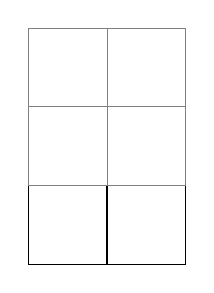
\begin{tikzpicture}[baseline=(current bounding box.east)]
  \draw (0,0) grid (2,1);
  \draw [help lines](0,1) grid (2,3);
\end{tikzpicture}
&
\begin{tikzcode}{}
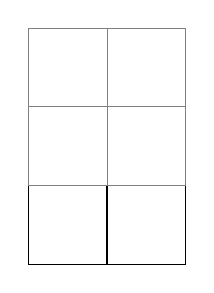
\begin{tikzpicture}
  \draw (0,0) grid (2,1);
  \draw [help lines](0,1) grid (2,3);
\end{tikzpicture}
\end{tikzcode}
\end{tabular}

点命令也非常好理解。其中\verb+\coordinate+是真正将点的名字和坐标联系起来的命令(相当于``赋值''),而\verb+\node+命令仅是一个标注文本的作用。

注意到第二行\verb+\node+命令,它使得字母B标注在pB点315度的位置。这样的效果往往优于其上一行的\verb+\node+命令的效果。注意:\RED{不要忘记{\texttt{\char92{}node}}命令后面的花括号(即使它是空的)}!

\noindent\begin{tabular}{p{0.25\linewidth}l}
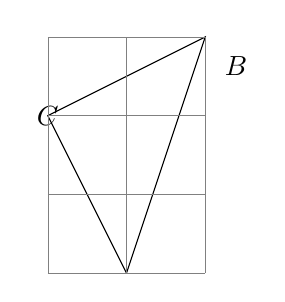
\begin{tikzpicture}[baseline=(current bounding box.east)]
  \coordinate (pA) at (1,0);
  \coordinate (pB) at (2,3);
  \coordinate (pC) at (0,2);
  \node at (pC) {$C$};
  \node[label=315:$B$] at (pB){};
  \draw (pA) -- (pB) -- (pC) -- (pA);
  \draw [help lines](0,0) grid (2,3);
\end{tikzpicture}
&
\begin{tikzcode}{}
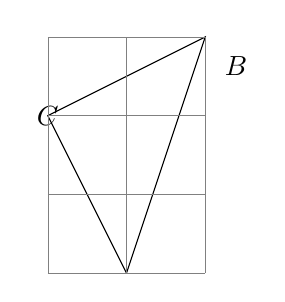
\begin{tikzpicture}
  \coordinate (pA) at (1,0);
  \coordinate (pB) at (2,3);
  \coordinate (pC) at (0,2);
  \node at (pC) {$C$};
  \node[label=315:$B$] at (pB){}; 
  \draw (pA) -- (pB) -- (pC) -- (pA);
  \draw [help lines](0,0) grid (2,3);
\end{tikzpicture}
\end{tikzcode}
\end{tabular}

\subsection{拉伸}
拉伸只需要在tikzpicture后添加xscale/yscale/scale的可选参数赋值即可。例如:

\noindent\begin{tabular}{p{0.25\linewidth}l}
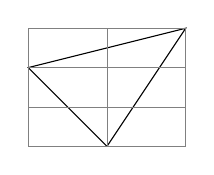
\begin{tikzpicture}[baseline=(current bounding box.east),yscale=0.5]
  \coordinate (pA) at (1,0);
  \coordinate (pB) at (2,3);
  \coordinate (pC) at (0,2);
  \draw (pA) -- (pB) -- (pC) -- (pA);
  \draw [help lines](0,0) grid (2,3);
\end{tikzpicture}
&
\begin{tikzcode}{}
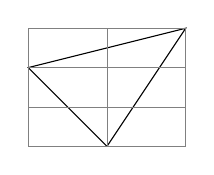
\begin{tikzpicture}[yscale=0.5]
  \coordinate (pA) at (1,0);
  \coordinate (pB) at (2,3);
  \coordinate (pC) at (0,2);
  \draw (pA) -- (pB) -- (pC) -- (pA);
  \draw [help lines](0,0) grid (2,3);
\end{tikzpicture}
\end{tikzcode}
\end{tabular}

\subsection{线宽}
线宽可以在tikzpicture后使用``[line width=5pt]''之类的参数进行\RED{全局调整},也可以在每个draw指令下分别地进行调整:

\noindent\begin{tabular}{p{0.25\linewidth}l}
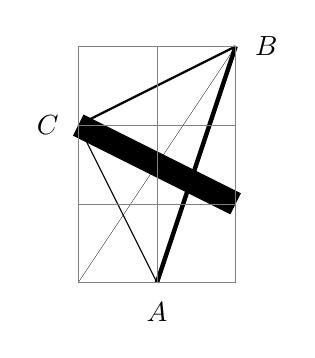
\begin{tikzpicture}[baseline=(current bounding box.east)]
  \coordinate (pA) at (1,0);
  \coordinate (pB) at (2,3);
  \coordinate (pC) at (0,2);
  \node[label=270:$A$] at (pA){};
  \node[label=0:$B$] at (pB){};
  \node[label=180:$C$] at (pC){};
  \draw[ultra thick] (pA) -- (pB);
  \draw[thick] (pB)-- (pC);
  \draw[thin] (pC)-- (pA);
  \draw[ultra thin] (pB) -- (0,0);
  \draw[line width=0.3cm] (pC) -- (2,1);
  \draw [help lines](0,0) grid (2,3);
\end{tikzpicture}
&
\begin{tikzcode}{}
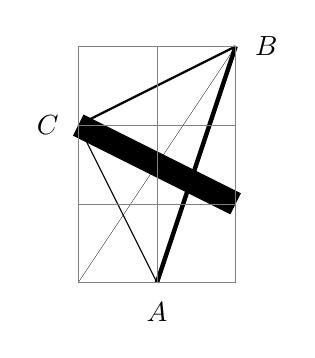
\begin{tikzpicture}
  \coordinate (pA) at (1,0);
  \coordinate (pB) at (2,3);
  \coordinate (pC) at (0,2);
  \node[label=270:$A$] at (pA){};
  \node[label=0:$B$] at (pB){};
  \node[label=180:$C$] at (pC){};
  \draw[ultra thick] (pA) -- (pB);
  \draw[thick] (pB)-- (pC);
  \draw[thin] (pC)-- (pA);
  \draw[ultra thin] (pB) -- (0,0);
  \draw[line width=0.3cm] (pC) -- (2,1);
  \draw [help lines](0,0) grid (2,3);
\end{tikzpicture}
\end{tikzcode}
\end{tabular}

\subsection{填色}
填色的逻辑非常简单,是指向绘制的\qd{闭合}图形内部填色。本例中,draw命令首尾相接地连接三个点,构成一个闭合图形——三角形,因此可以填色:

\noindent\begin{tabular}{p{0.25\linewidth}l}
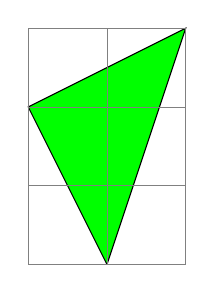
\begin{tikzpicture}[baseline=(current bounding box.east)]
  \coordinate (pA) at (1,0);
  \coordinate (pB) at (2,3);
  \coordinate (pC) at (0,2);
  \draw[fill=green] (pA) -- (pB) -- (pC) -- (pA);
  \draw[help lines](0,0) grid (2,3);
\end{tikzpicture}
&
\begin{tikzcode}{}
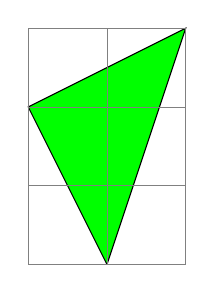
\begin{tikzpicture}
  \coordinate (pA) at (1,0);
  \coordinate (pB) at (2,3);
  \coordinate (pC) at (0,2);
  \draw[fill=green] (pA) -- (pB) -- (pC) -- (pA);
  \draw[help lines] (0,0) grid (2,3);
\end{tikzpicture}
\end{tikzcode}
\end{tabular}

\subsection{点样式}
填色之后图形好看了许多,但是还不够。点标在图中似乎也不看清位置,不过这是有方法解决的:

\noindent\begin{tabular}{p{0.25\linewidth}l}
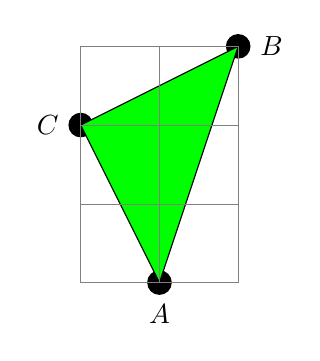
\begin{tikzpicture}[baseline=(current bounding box.east)]
  \coordinate (pA) at (1,0);
  \coordinate (pB) at (2,3);
  \coordinate (pC) at (0,2);
  \node[label=270:$A$,circle,draw,fill,inner sep=3pt] at (pA){};
  \node[label=0:$B$,circle,draw,fill,inner sep=3pt] at (pB){};
  \node[label=180:$C$,circle,draw,fill,inner sep=3pt] at (pC){};
  \draw[fill=green] (pA) -- (pB) -- (pC) -- (pA);
  \draw[help lines] (0,0) grid (2,3);
\end{tikzpicture}
&
\begin{tikzcode}{}
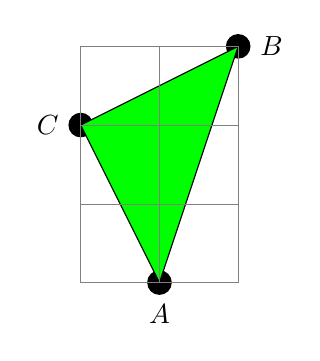
\begin{tikzpicture}
  \coordinate (pA) at (1,0);
  \coordinate (pB) at (2,3);
  \coordinate (pC) at (0,2);
  \node[label=270:$A$,circle,draw,fill,inner sep=3pt] at (pA){};
  \node[label=0:$B$,circle,draw,fill,inner sep=3pt] at (pB){};
  \node[label=180:$C$,circle,draw,fill,inner sep=3pt] at (pC){};
  \draw[fill=green] (pA) -- (pB) -- (pC) -- (pA);
  \draw[help lines] (0,0) grid (2,3);
\end{tikzpicture}
\end{tikzcode}
\end{tabular}

但是这一长串简直是太复杂了。大概能看懂circle是将点画成圆形,fill表示填充,inner sep表示点的大小。而Tikz给出的\verb+\tikzstyle+能够简化步骤。

还有一点就是,绿色的填充似乎位于点的上方?还是乖乖地调整语句顺序吧。

\noindent\begin{tabular}{p{0.25\linewidth}l}
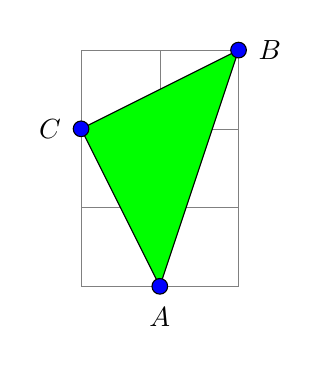
\begin{tikzpicture}[baseline=(current bounding box.east)]
  \draw[help lines] (0,0) grid (2,3);
  \coordinate (pA) at (1,0);
  \coordinate (pB) at (2,3);
  \coordinate (pC) at (0,2);
  \draw[fill=green] (pA) -- (pB) -- (pC) -- (pA);
  \tikzstyle{every node} = [circle,draw,fill=blue,inner sep=2pt];
  \node[label=270:$A$] at (pA){};
  \node[label=0:$B$] at (pB){};
  \node[label=180:$C$] at (pC){};   
\end{tikzpicture}
&
\begin{tikzcode}{}
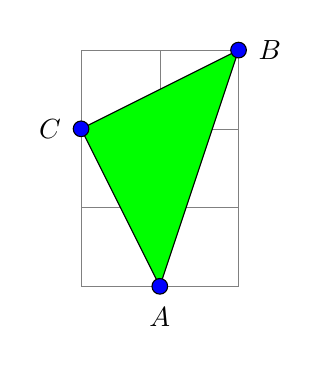
\begin{tikzpicture}
  \draw[help lines] (0,0) grid (2,3);
  \coordinate (pA) at (1,0);
  \coordinate (pB) at (2,3);
  \coordinate (pC) at (0,2);
  \draw[fill=green] (pA) -- (pB) -- (pC) -- (pA);
  \tikzstyle{every node} = [circle,draw,fill=blue,inner sep=2pt];
  \node[label=270:$A$] at (pA){};
  \node[label=0:$B$] at (pB){};
  \node[label=180:$C$] at (pC){}; 
\end{tikzpicture}
\end{tikzcode}
\end{tabular}

注意:\verb+\tikzstyle{every node}+控制的是其下方代码的所有node的点样式,不影响其上方代码中的点。

\subsection{线型和颜色}
除了点的定义,线当然也可以定义。线型有dashed/dotted两种,颜色除了默认的也可以通过叹号的形式控制。

\noindent\begin{tabular}{p{0.25\linewidth}l}
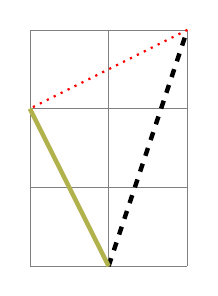
\begin{tikzpicture}[baseline=(current bounding box.east)]
  \draw[help lines] (0,0) grid (2,3);
  \coordinate (pA) at (1,0);
  \coordinate (pB) at (2,3);
  \coordinate (pC) at (0,2);
  \draw[dashed, ultra thick] (pA) -- (pB);
  \draw[dotted, red, thick] (pB) -- (pC);
  \draw[blue!30!yellow, ultra thick] (pC) -- (pA);
\end{tikzpicture}
&
\begin{tikzcode}{}
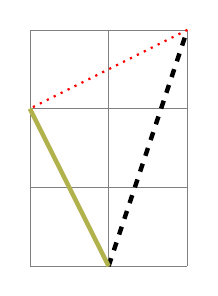
\begin{tikzpicture}
  \draw[help lines] (0,0) grid (2,3);
  \coordinate (pA) at (1,0);
  \coordinate (pB) at (2,3);
  \coordinate (pC) at (0,2);
  \draw[dashed, ultra thick] (pA) -- (pB);
  \draw[dotted, red, thick] (pB) -- (pC);
  \draw[blue!30!yellow, ultra thick] (pC) -- (pA);
\end{tikzpicture}
\end{tikzcode}
\end{tabular}

主要的颜色包括\footnote{以下色块用\texttt{\char92{}tikz\{\char92{}draw[{\it color},line width=9] (0,0) -- (0.5,0);\}绘制得到。}}:
\tikzline{red}\tikzline{green}\tikzline{yellow}\tikzline{blue}\tikzline{cyan}
\tikzline{magenta}\tikzline{black}\tikzline{gray}\tikzline{darkgray}\tikzline{lightgray}
\tikzline{brown}\tikzline{lime}\tikzline{olive}\tikzline{orange}\tikzline{pink}\tikzline{purple}
\tikzline{teal}\tikzline{violet}
还有white\tikz{\draw[white,line width=9](0,0)--(0.5,0);}.

\subsection{箭头}
箭头也是需要经常绘制的内容。主要也是根据\verb+\draw+命令的参数控制:

\noindent\begin{tabular}{p{0.25\linewidth}l}
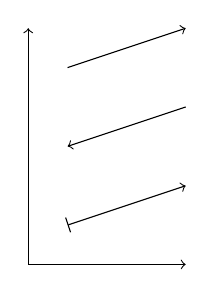
\begin{tikzpicture}[baseline=(current bounding box.east)]
  \draw[->] (0.5,2.5) -- (2,3);
  \draw[<-] (0.5,1.5) -- (2,2);
  \draw[|->] (0.5,0.5)-- (2,1); 
  \draw[<->] (0,3) -- (0,0) -- (2,0);
\end{tikzpicture}
&
\begin{tikzcode}{}
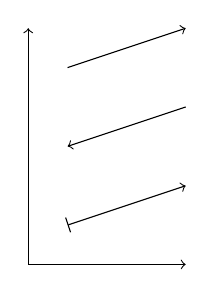
\begin{tikzpicture}
  \draw[->] (0.5,2.5) -- (2,3);
  \draw[<-] (0.5,1.5) -- (2,2);
  \draw[|->] (0.5,0.5)-- (2,1); 
  \draw[<->] (0,3) -- (0,0) -- (2,0);
\end{tikzpicture}
\end{tikzcode}
\end{tabular}

\section{高效书写}
\subsection{变量}
变量申请使用与\LaTeX 相同的语句:\verb+\newcommand+. 注意:变量需要以反斜杠开头,并与现有命令不重复。

\noindent\begin{tabular}{p{0.25\linewidth}l}
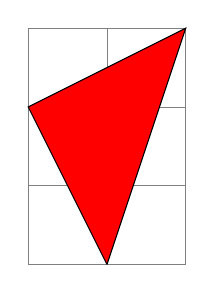
\begin{tikzpicture}[baseline=(current bounding box.east)]
  \draw [help lines](0,0) grid (2,3);
  \newcommand{\aaa}{1};
  \newcommand{\bbb}{3};
  \newcommand{\ccc}{2};
  \coordinate (pA) at (\aaa,0);
  \coordinate (pB) at (\ccc,\bbb);
  \coordinate (pC) at (0,\ccc);
  \draw[fill=red] (pA) -- (pB) -- (pC) -- (pA); 
\end{tikzpicture}
&
\begin{tikzcode}{}
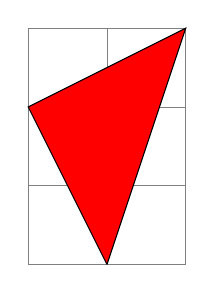
\begin{tikzpicture}
  \draw [help lines](0,0) grid (2,3);
  \newcommand{\aaa}{1};
  \newcommand{\bbb}{3};
  \newcommand{\ccc}{2};
  \coordinate (pA) at (\aaa,0);
  \coordinate (pB) at (\ccc,\bbb);
  \coordinate (pC) at (0,\ccc);
  \draw[fill=red] (pA) -- (pB) -- (pC) -- (pA); 
\end{tikzpicture}
\end{tikzcode}
\end{tabular}

\subsection{循环}
但是同样的语句书写很多遍是很复杂的,好在Tikz提供了循环的实现方法:

\noindent\begin{tabular}{p{0.25\linewidth}l}
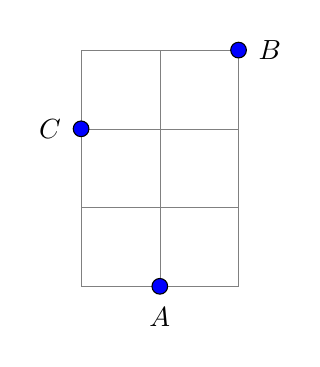
\begin{tikzpicture}[baseline=(current bounding box.east)]
  \newcommand{\la}{1};
  \newcommand{\lb}{3};
  \newcommand{\lc}{2};
  \draw [help lines](0,0) grid (\lc,\lb);
  \coordinate (pA) at (\la,0);
  \coordinate (pB) at (\lc,\lb);
  \coordinate (pC) at (0,\lc);
  \tikzstyle{every node}=[circle, draw, fill=blue,inner sep=2pt];
  \foreach \x/\y in {A/270,B/0,C/180}{
    \node[label=\y:$\x$] at (p\x){};
  }
\end{tikzpicture}
&
\begin{tikzcode}{}
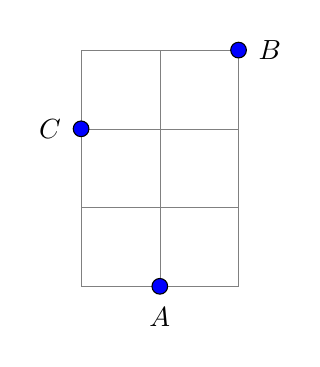
\begin{tikzpicture}
  \newcommand{\la}{1};
  \newcommand{\lb}{3};
  \newcommand{\lc}{2};
  \draw [help lines](0,0) grid (\lc,\lb);
  \coordinate (pA) at (\la,0);
  \coordinate (pB) at (\lc,\lb);
  \coordinate (pC) at (0,\lc);
  \tikzstyle{every node}=[circle, draw, fill=blue,inner sep=2pt];
  \foreach \x/\y in {A/270,B/0,C/180}{
    \node[label=\y:$\x$] at (p\x){};
  }
\end{tikzpicture}
\end{tikzcode}
\end{tabular}

注意到:甚至点的名称pA, pB, pC中的A, B, C也是可以通过foreach来指定的!

\subsection{运算}
\fbox{{\itshape{注意:需要在导言区添加}}\latexline{\\usetikzlibrary{calc}}。文中不再写出。}

如果一个绘图工具仅仅能够绘图而不能做运算……它有什么用呢?如果作为科学排版系统下的绘图工具而不支持运算的话,Tikz岂不是太弱了?

\noindent\begin{tabular}{p{0.25\linewidth}l}
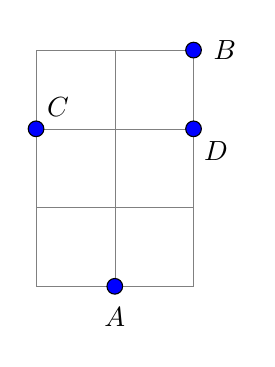
\begin{tikzpicture}[baseline=(current bounding box.east)]
  \draw [help lines](0,0) grid (2,3);
  \coordinate (pA) at (1,0);
  \coordinate (pB) at (2,3);
  \coordinate (pC) at (0,2);
  \coordinate (pD) at ($(pB)+(0,-1)$);
  \tikzstyle{every node}=[circle, draw, fill=blue,inner sep=2pt];
  \foreach \x/\y in {A/270,B/0,C/45,D/315}{
    \node[label=\y:$\x$] at (p\x){};
  }
\end{tikzpicture}
&
\begin{tikzcode}{}
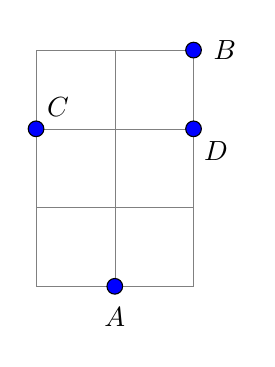
\begin{tikzpicture}
  \draw [help lines](0,0) grid (2,3);
  \coordinate (pA) at (1,0);
  \coordinate (pB) at (2,3);
  \coordinate (pC) at (0,2);
  \coordinate (pD) at ($(pB)+(0,-1)$);
  \tikzstyle{every node}=[circle, draw, fill=blue,inner sep=2pt];
  \foreach \x/\y in {A/270,B/0,C/45,D/315}{
    \node[label=\y:$\x$] at (p\x){};
  }
\end{tikzpicture}
\end{tikzcode}
\end{tabular}

\clearpage
\begin{appendices}
\renewcommand{\thechapter}{\Roman{chapter}}
\titleformat{\chapter}[display]{\Huge\bfseries}{附录\Alph{chapter}}{1em}{}
\renewcommand{\thesection}{\thechapter-\arabic{section}}
\titleformat{\section}[hang]{\bfseries\Large}{\S\ \thesection}{1em}{}{}

\chapter{注音符号}
\begin{center}
\tabcaption{注音符号与特殊符号}
\begin{tabular}{|p{4em}<{\centering} @{-\hspace{1em}} p{3em}|p{4em}<{\centering} @{-\hspace{1em}} p{3em}|p{4em}<{\centering} @{-\hspace{1em}} p{3em}|p{4em}<{\centering} @{-\hspace{1em}} p{3em}|}
\hline
\textbf{样式} & \textbf{命令} & \textbf{样式} & \textbf{命令} & \textbf{样式} & \textbf{命令} & \textbf{样式} & \textbf{命令}\\
\hline
\=o  & \verb|\=o|  & \'o  & \verb|\'o|  & \v o & \verb|\v o|  & \`o   & \verb|\`o|  \\
\^o  & \verb|\^o|  & \"o  & \verb|\"o|  & \.o  & \verb|\.o|   & \H o  & \verb|\H o| \\
\d o & \verb|\d o| & \u o & \verb|\u o| & \b o & \verb|\b o|  & \t oo & \verb|\t oo|\\
\multicolumn{2}{|c@{\bf --}}{$\tilde{o}$} & \multicolumn{2}{@{\bf --}c|}{\tt{\$$\backslash$tilde\{o\}\$}} &%
\multicolumn{2}{c@{\bf --}}{$\hat{o}$}    & \multicolumn{2}{@{\bf --}c|}{\tt{\$$\backslash$hat\{o\}\$}}\\
\o  & \verb|\o|  & \O  & \verb|\O|  & \i  & \verb|\i|  & \j  & \verb|\j| \\
\multicolumn{8}{|c|}{}\\
\aa & \verb|\aa| & \AA & \verb|\AA| & \ae & \verb|\ae| & \AE & \verb|\AE|\\
\oe & \verb|\oe| & \OE & \verb|\OE| & !`  & \verb|!`|  & ?`  & \verb|?`| \\
\hline
\end{tabular}
\end{center}

\end{appendices}

\end{document}
